
Because it includes an on-shell Z boson as well as a b-jet and W from the top decay, tZ production represents an identical final state  to WZ + b-jet. This implies the possibility of matrix level interference between these two processes not accounted for in the Monte Carlo simulations, which consider the two processes independently. Truth level studies are performed in order to estimate the impact of these interference effects.

Because tZ produces a final state identical to signal, it represents a predominant background in the most signal enriched regions. Therefore, a boosted decision tree (BDT) algorithm is trained using TMVA \cite{TMVA_guide} to separate $WZ$ + heavy flavor from tZ.

Separation between tZ and $WZ$ + heavy flavor is achieved in part by reconstructing the invariant mass of the top candidate, which clusters more closely to the top mass for tZ than WZ + heavy flavor.

The result of this BDT is used to create a tZ enriched region in the fit, reducing its impact on the measurement of WZ + heavy flavor.

\subsection{Interference Studies}
\label{subsec:interference}

In order to estimate the matrix level interference effects between tZ and WZ + b-jet, two different sets of simulations are produced using MadGraph 5 \cite{Madgraph} - one which simulates these two processes independently, and another where they are produced simultaneously, such that interference effects are present. These two sets of samples are then compared, and the difference between them can be taken to represent any interference effects.

MadGraph simulations of 10,000 tZ and 10,000 WZ + b-jet events are produced, along with 20,000 events where both are present, in the fiducial region where three leptons and at least one jet are produced. 

The kinematics of these samples are shown below:

\begin{figure}[H]
    \subfigure[]{\includegraphics[width=.47\linewidth]{tZInterference/lepPairMass23.eps}}%
    \subfigure[]{\includegraphics[width=.47\linewidth]{tZInterference/lep1pt.eps}}\\                        
    \subfigure[]{\includegraphics[width=.47\linewidth]{tZInterference/drll23.eps}}%
    \subfigure[]{\includegraphics[width=.47\linewidth]{tZInterference/btpt.eps}}\\
    \caption{Comparisons between (a) the invariant mass of the Z-candidate, (b) the $p_T$ of the leading lepton, (c) $\Delta(R)$ of the two leptons that form the Z-candidate, and (d) the $p_T$ of the b-jet, for WZ and tZ events generated with interference effects (blue) and without interference effects (red).}
\end{figure}

%\begin{figure}[H]
%\end{figure}

\subsection{Top Mass Reconstruction}
\label{subsec:topMass}

 The reconstruction of the top mass follows the procedure described in detail in section 6.1 of \cite{ttZ_paper}. The mass of the top quark candidate is reconstructed from the jet, the lepton not included in the Z-candidate, and a reconstructed neutrino. Since the selection requires exactly one jet in the event, there is only possible b-jet candidate. 

The neutrino from the W decay is expected to be the only source of $E_T^{miss}$. Therefore, the $E_T$ and $\phi$ of the neutrino are taken from the $E_T^{miss}$ measurement. This leaves the z-component of the neutrino momentum, $p_{\nu z}$ as the only unknown.

This unknown is solved for by taking the combined invariant mass of the lepton and neutrino to give the invariant mass of the $W$ boson:

\begin{center}
   $(p_l + p_{\nu})^2 = m_W^2$ \\ 
\end{center} 

Expanding this out into components, this equation gives:

\begin{center}
   $\sqrt{p_{T\nu^2}+p_{z\nu^2}}E_l = \frac{m^2_w-m^2_l}{2}+p_{T\nu}(p_{lx} cos\phi_\nu + p_{ly} sin \phi_\nu) + p_{lz} p_{\nu z}$ \\ 
\end{center} 

This equation gives two solutions for $p_{\nu z}$. For cases where only one of these solutions is real, that is taken as the value of $p_{\nu z}$. For instances with two real solutions, the one which is shown to be correct in the largest fraction of simulations is taken. For cases when no real solution is found, often because of detector effects, the value of $E_T^{miss}$ is varied in decreasing increments of 100 MeV until a real solution is found.

The reconstructed top mass distribution for tZ and $WZ$ + b can be seen in figure \ref{fig:topMass}.

\begin{figure}
    \centering
    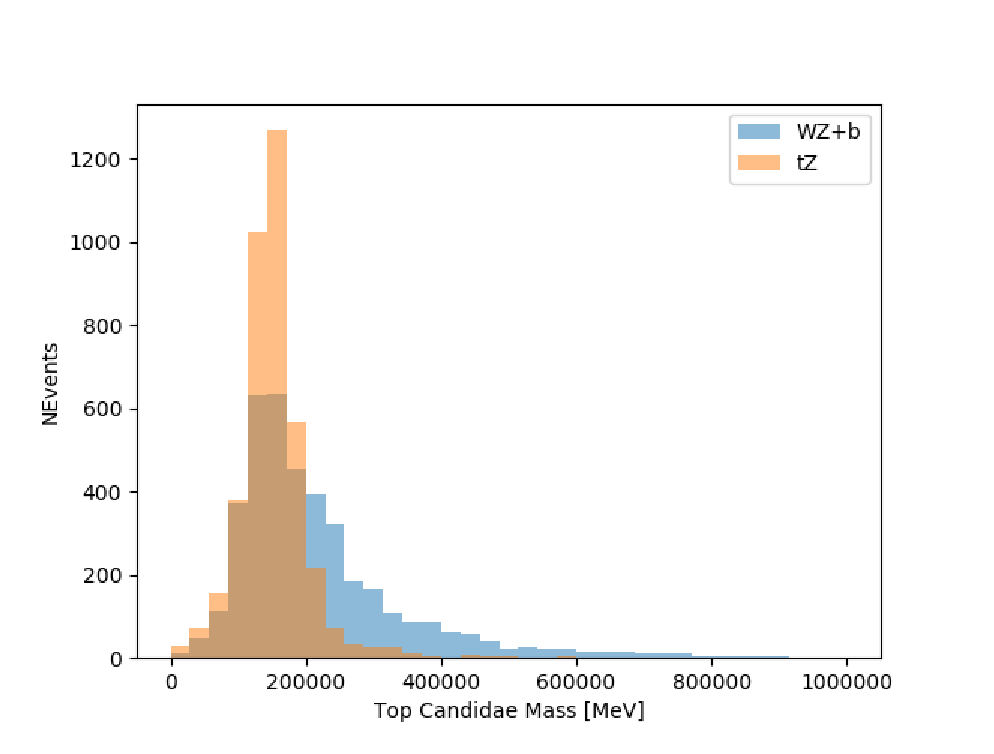
\includegraphics[width=0.7\linewidth]{tZ_bdt/topMass.eps}
    \caption{Reconstructed top mass distributions for tZ and $WZ$ + b, measured in MeV.}
    \label{fig:topMass}
\end{figure}

\subsection{tZ BDT}
\label{subsec:tZ_bdt}
 
A Boosted Decision Tree (BDT), specifically XGBoost \cite{xgboost_cite}, is used to provide separation between tZ and WZ+b. The following kinematic variables are used as inputs:
 
 \begin{itemize}
     \item The invariant mass of the reconstructed top candidate
     \item $p_T$ of each of the leptons, jet
     \item The  invariant mass of each combination of lepton pairs, $M(ll)$
     \item $E_T^{miss}$
     \item Distance between each combination of leptons, $\Delta R (ll)$
     \item Distance between each lepton and the jet, $\Delta R (lj)$
 \end{itemize}
 
The training samples included only events meeting the requirements of the 1-jet, >60\% region, i.e. passing all the selection described in section \ref{sec:evt_selection} and having exactly one jet which passes the tightest (60\%) DL1r working point.
 
The distributions of a few of these features for both signal and background is shown in figure \ref{fig:tZ_kinematics}.
 
\begin{figure}[h!]
\center
    \subfigure[]{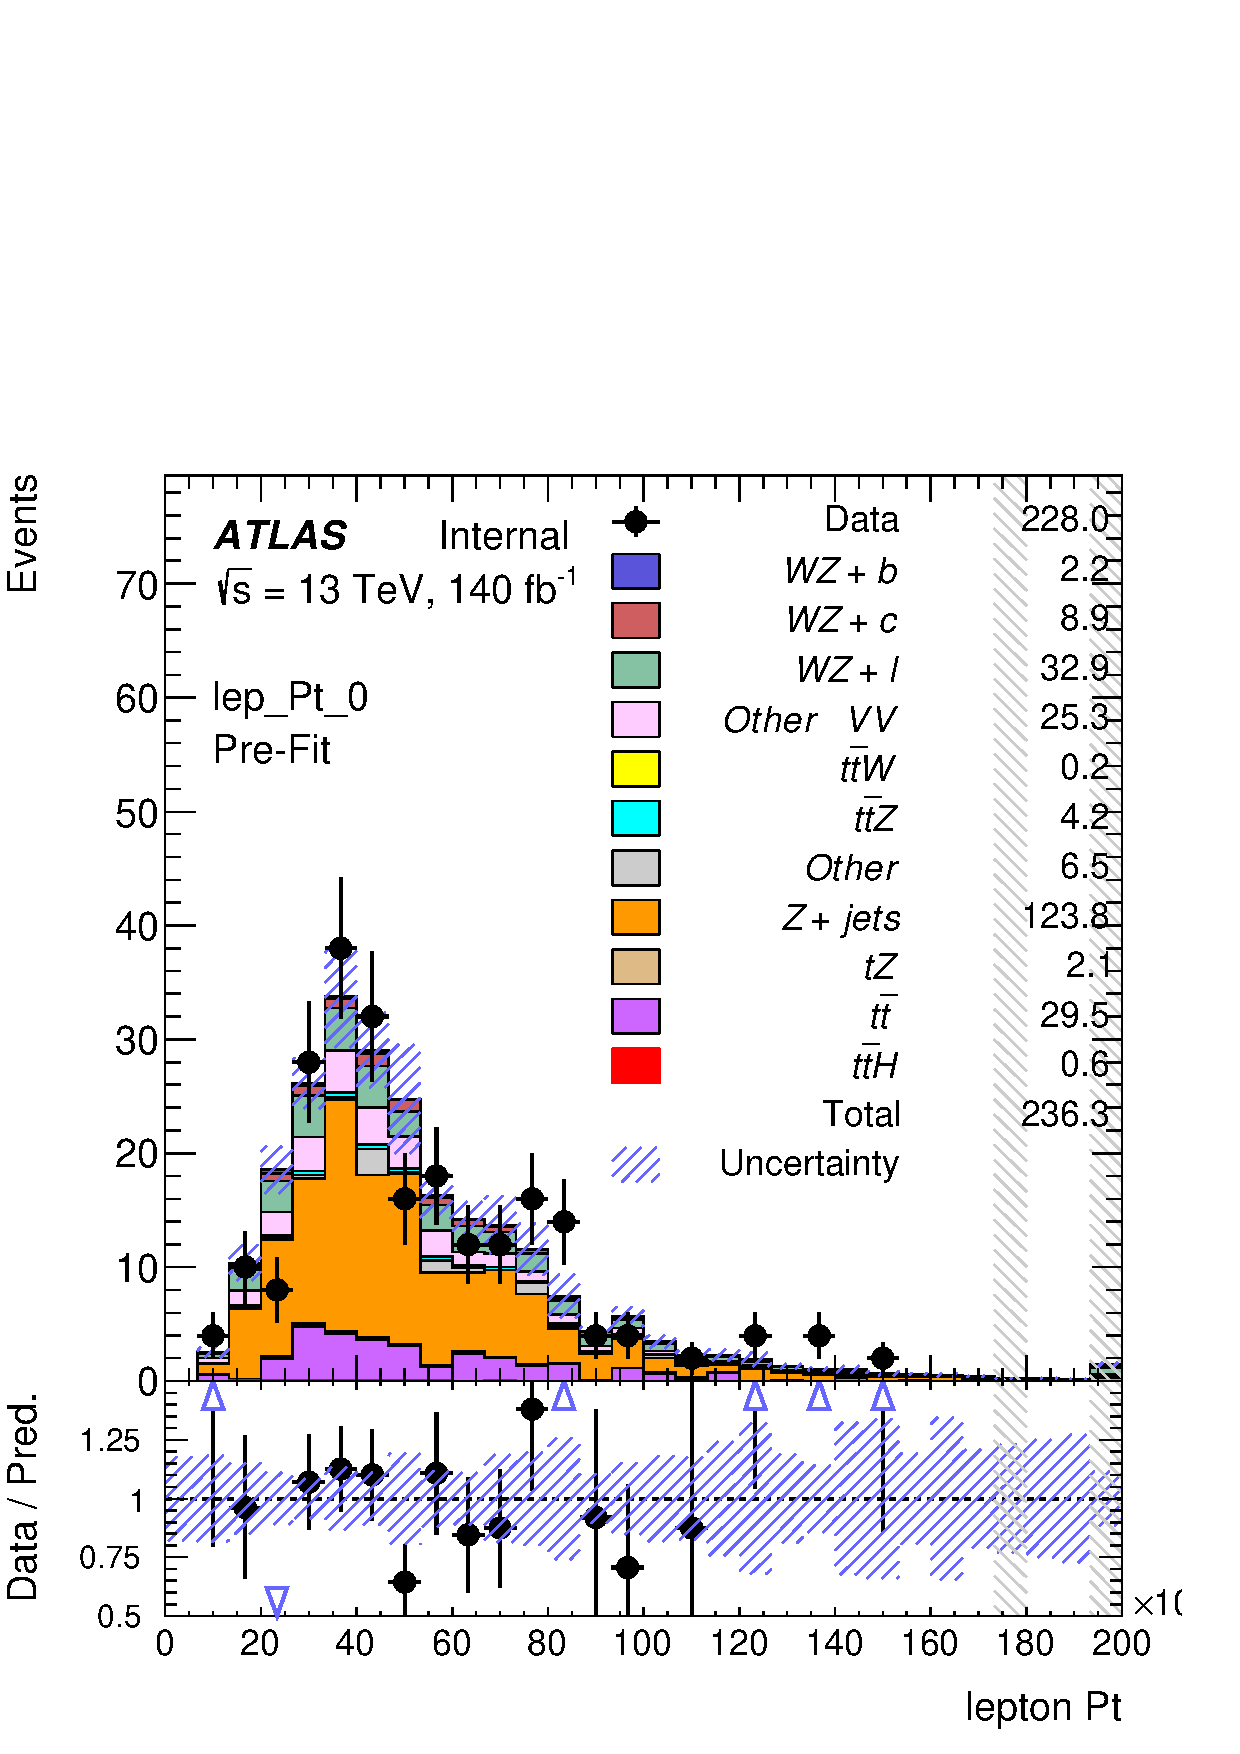
\includegraphics[width=.32\linewidth]{tZ_bdt_ab127/1j/ab127/lep_Pt_0.pdf}}%
    \subfigure[]{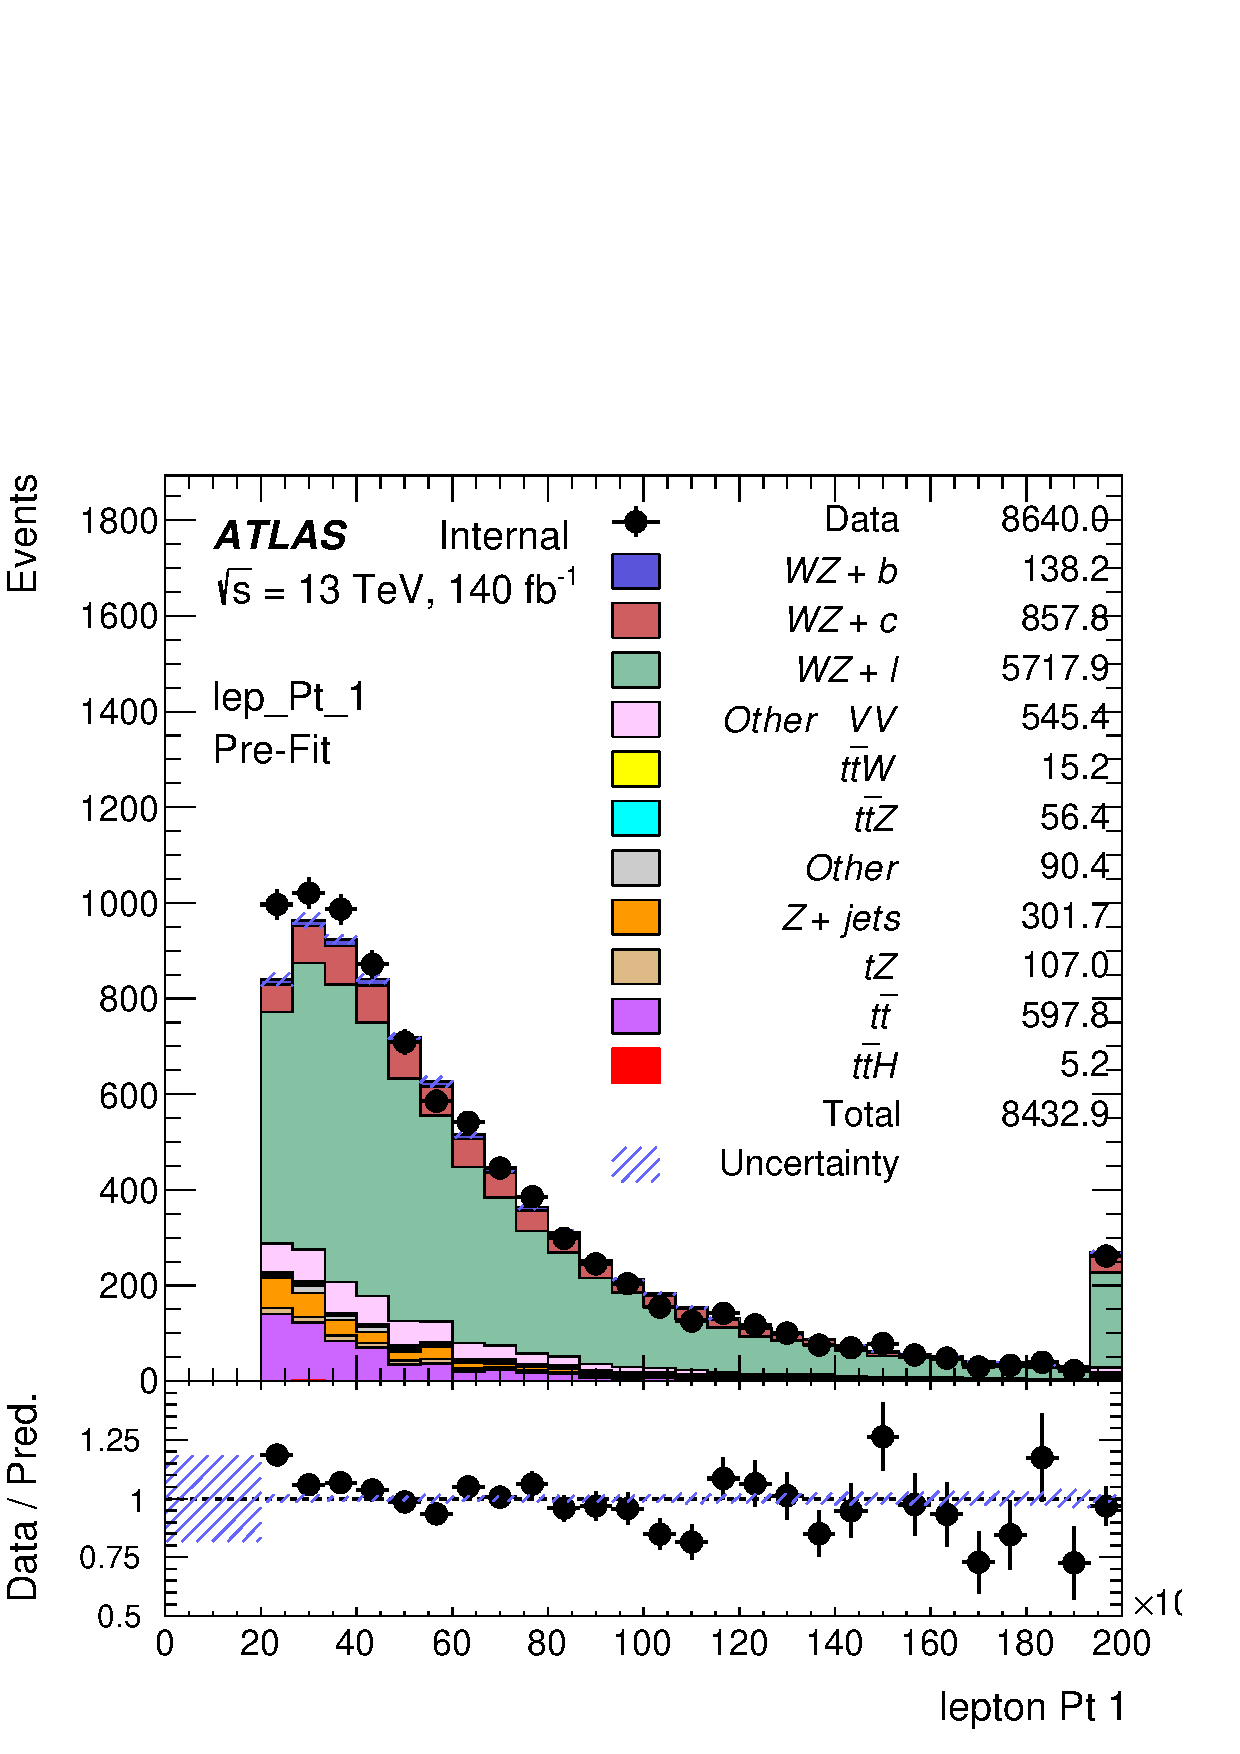
\includegraphics[width=.32\linewidth]{tZ_bdt_ab127/1j/ab127/lep_Pt_1.pdf}}%
    \subfigure[]{\includegraphics[width=.32\linewidth]{tZ_bdt_ab127/1j/ab127/jet_Pt_0.pdf}}\\
    \subfigure[]{\includegraphics[width=.32\linewidth]{tZ_bdt_ab127/1j/ab127/topMassReco.pdf}}% 
    \subfigure[]{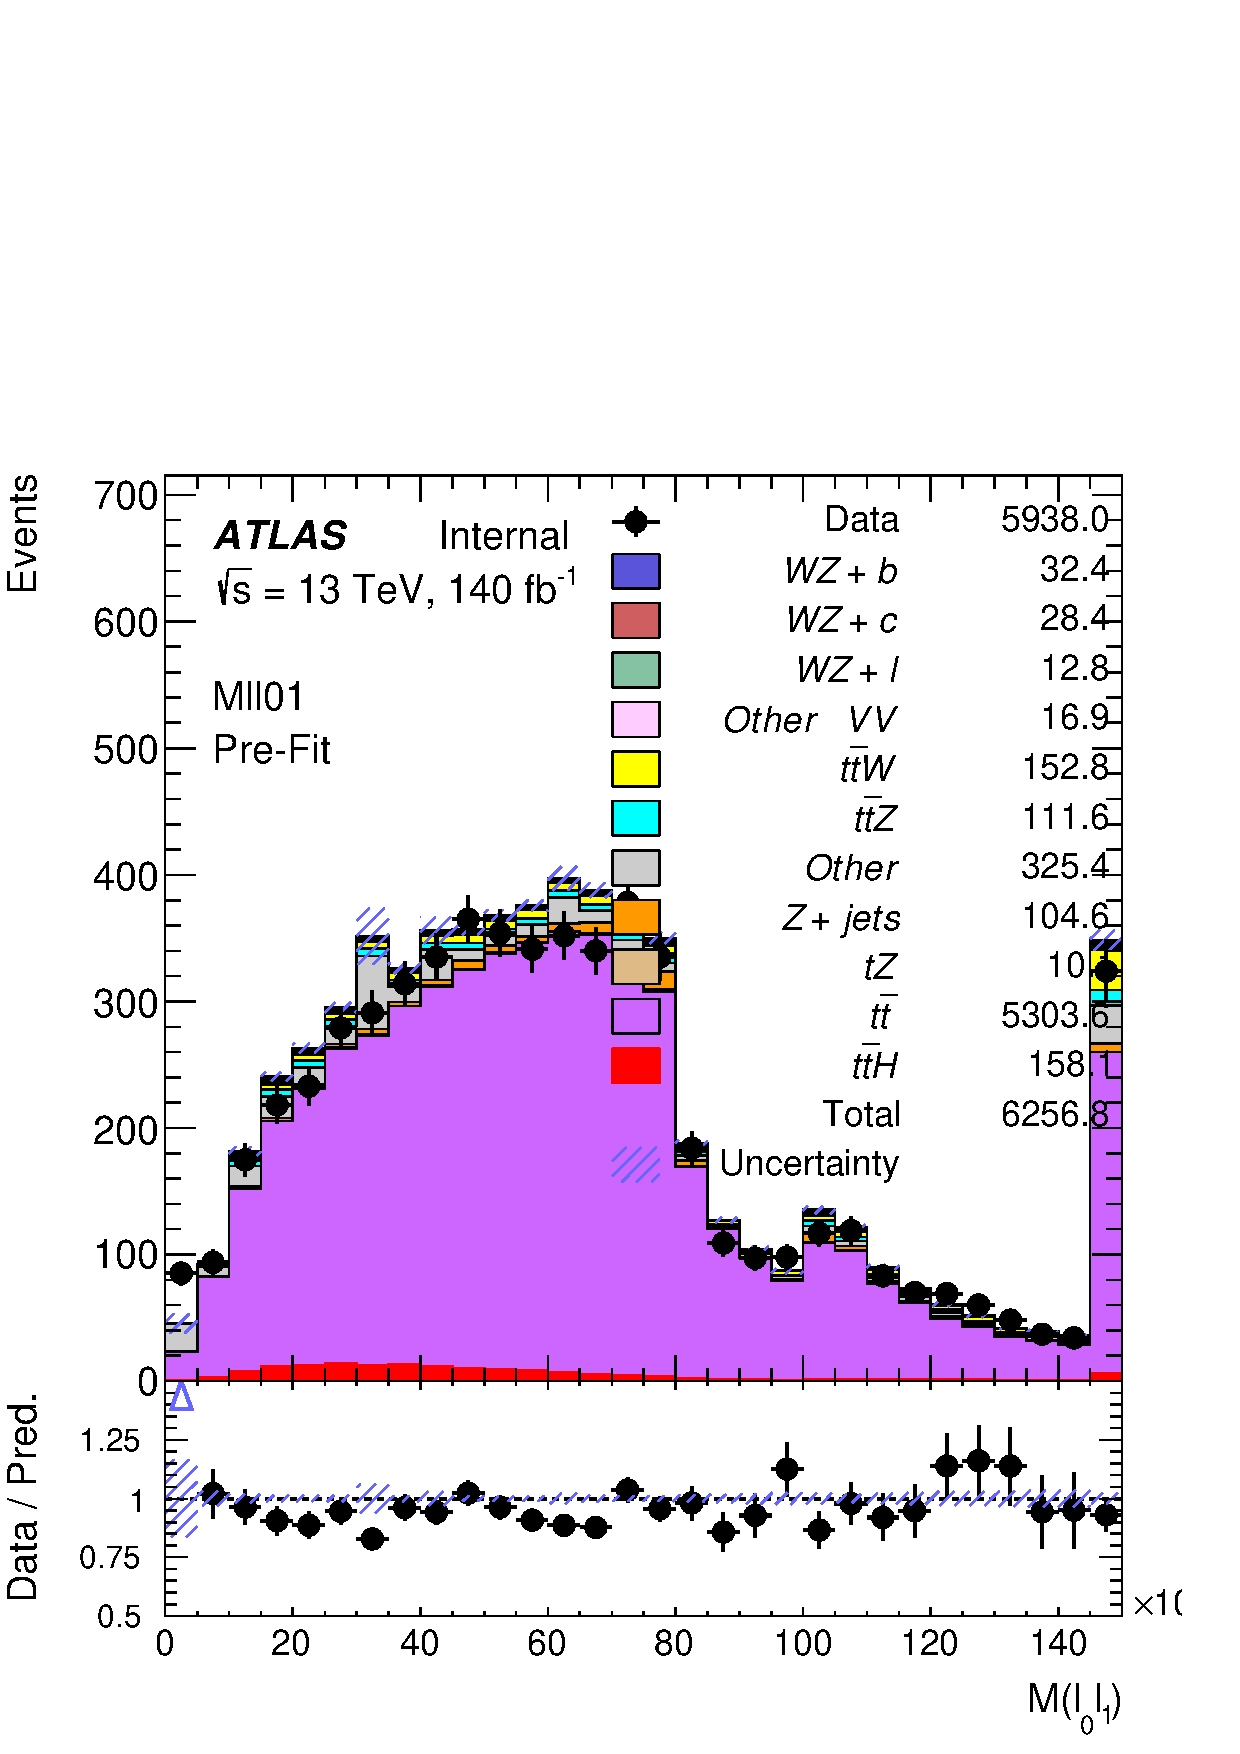
\includegraphics[width=.32\linewidth]{tZ_bdt_ab127/1j/ab127/Mll01.pdf}}%
    \subfigure[]{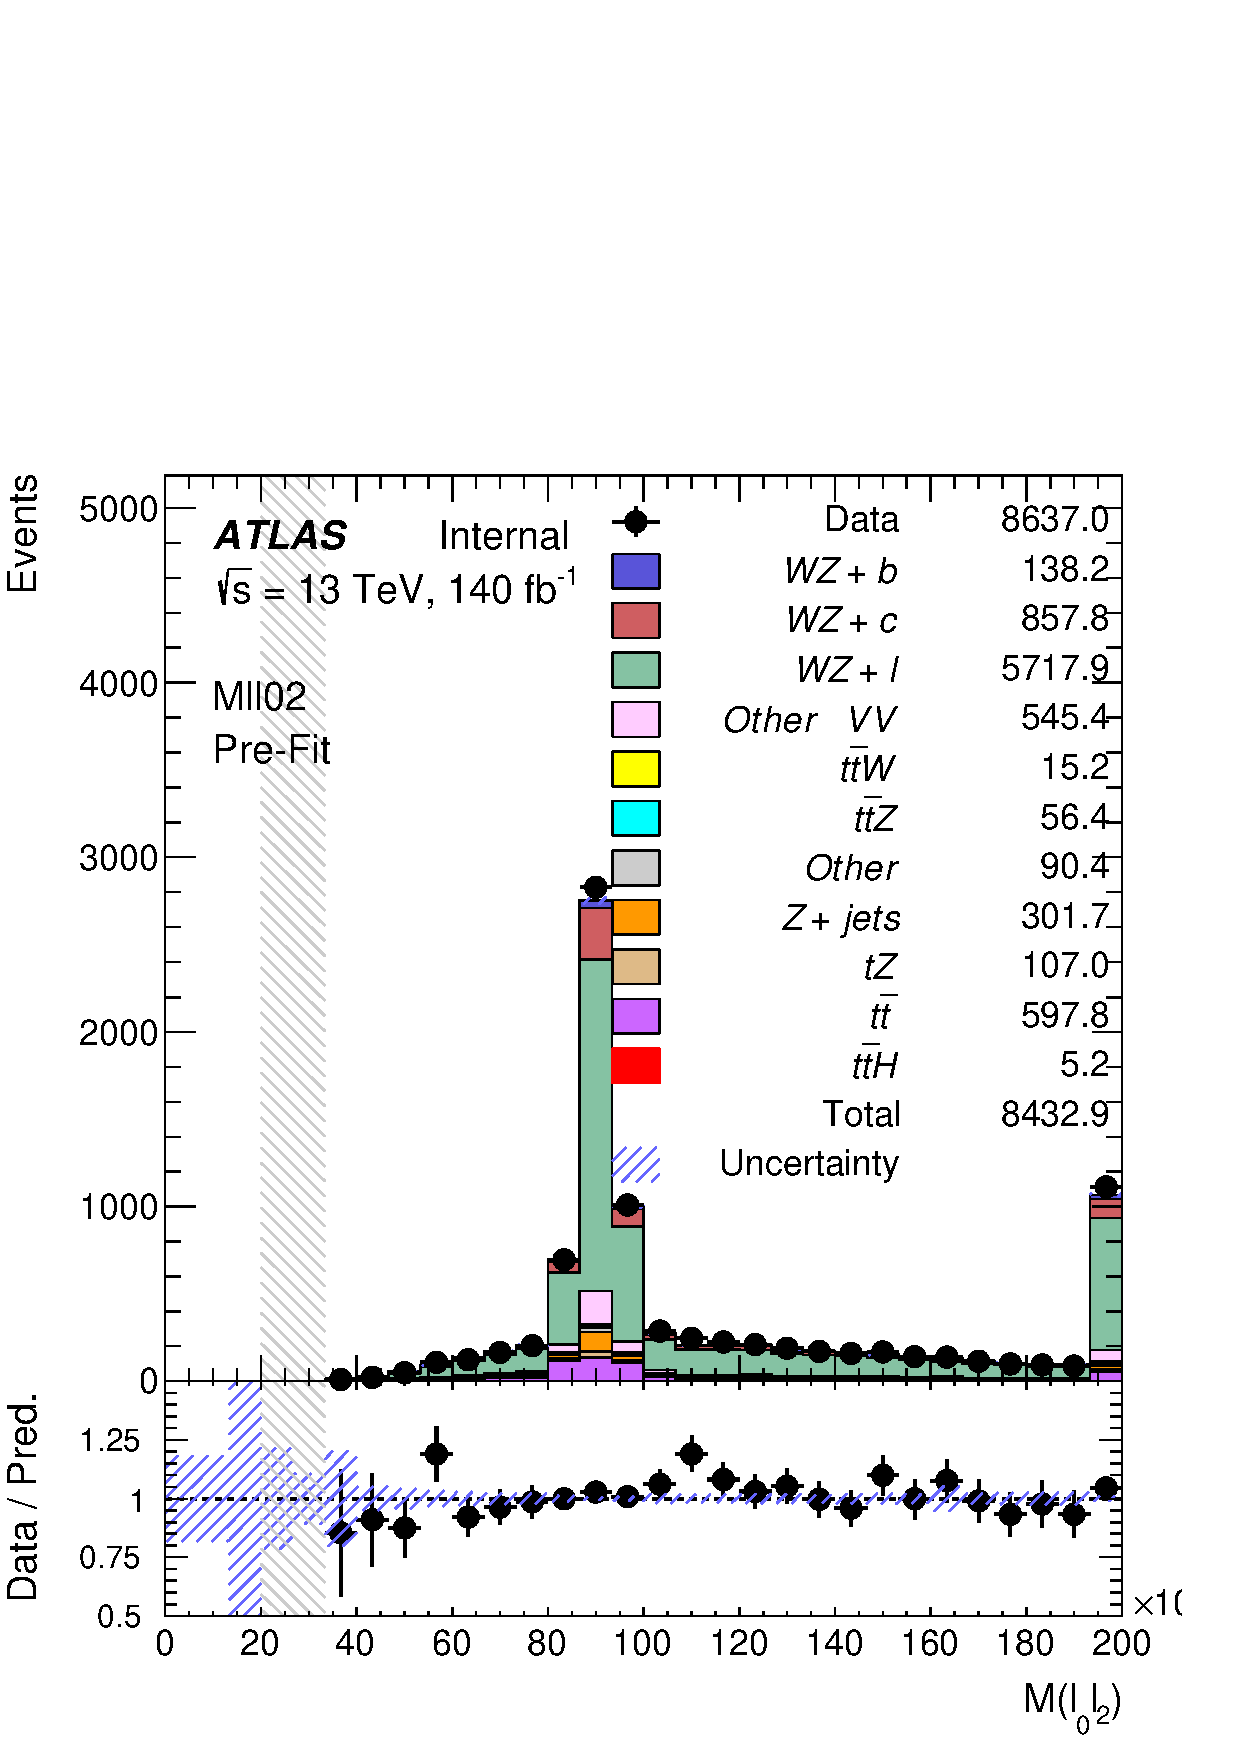
\includegraphics[width=.32\linewidth]{tZ_bdt_ab127/1j/ab127/Mll02.pdf}}\\
    \subfigure[]{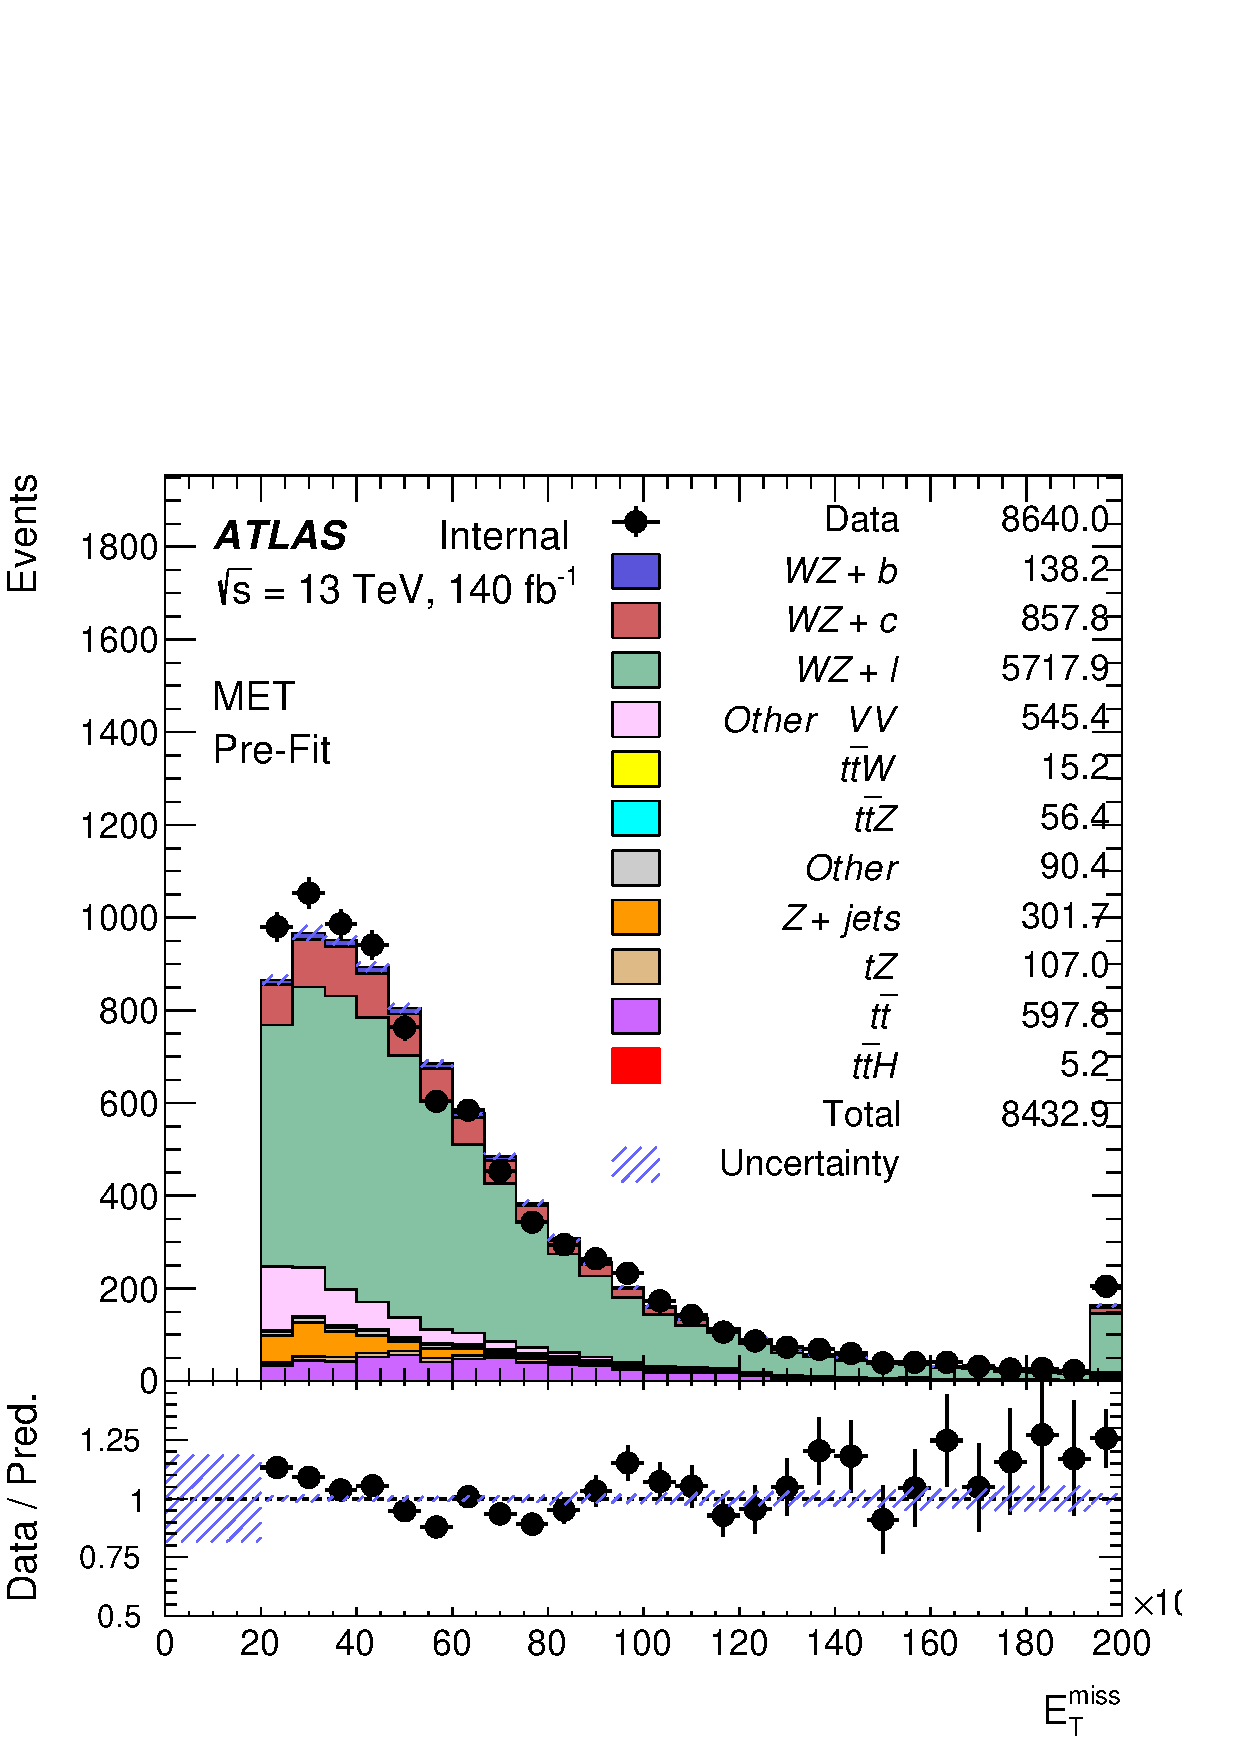
\includegraphics[width=.32\linewidth]{tZ_bdt_ab127/1j/ab127/MET.pdf}}%                           
    \subfigure[]{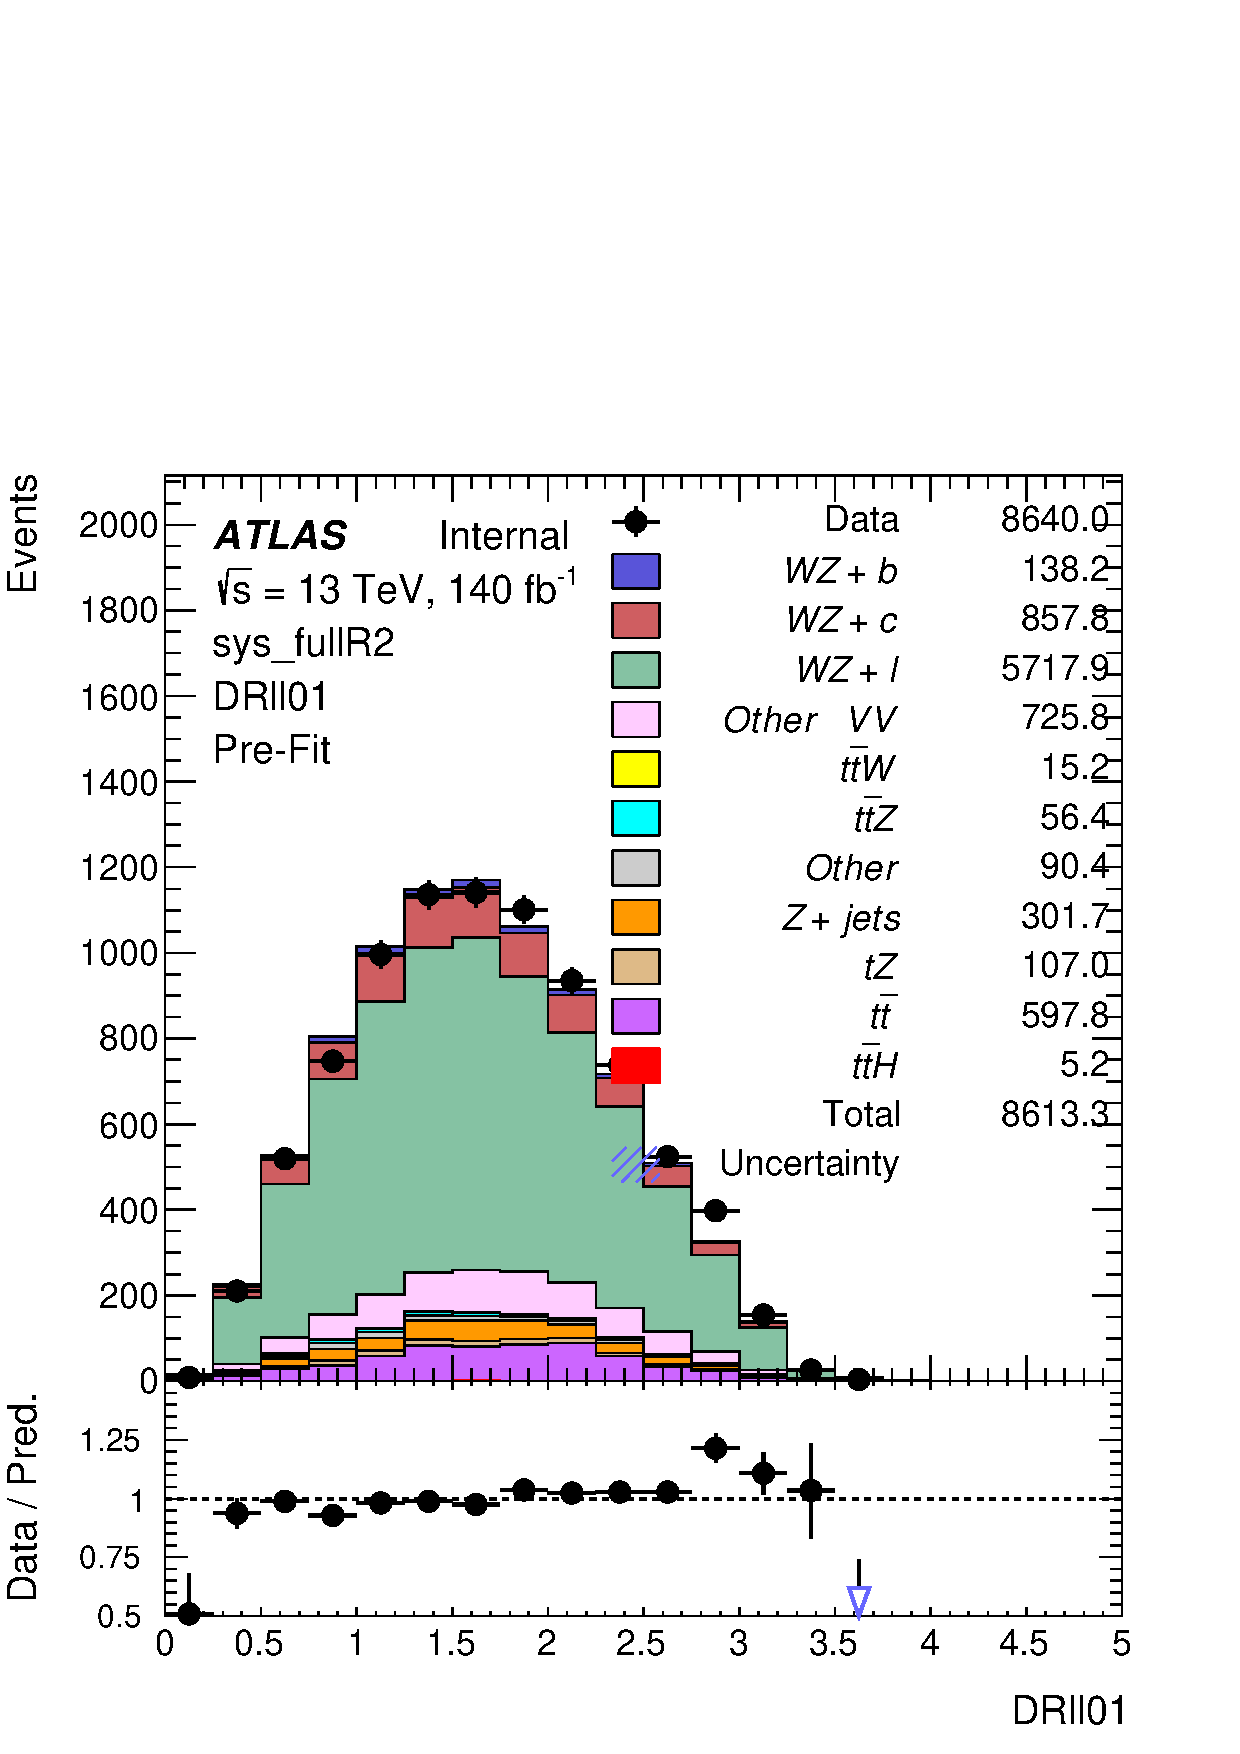
\includegraphics[width=.32\linewidth]{tZ_bdt_ab127/1j/ab127/DRll01.pdf}}%                                  
    \subfigure[]{\includegraphics[width=.32\linewidth]{tZ_bdt_ab127/1j/ab127/minDeltaR_LJ_0.pdf}}\\                          
    %\subfigure[]{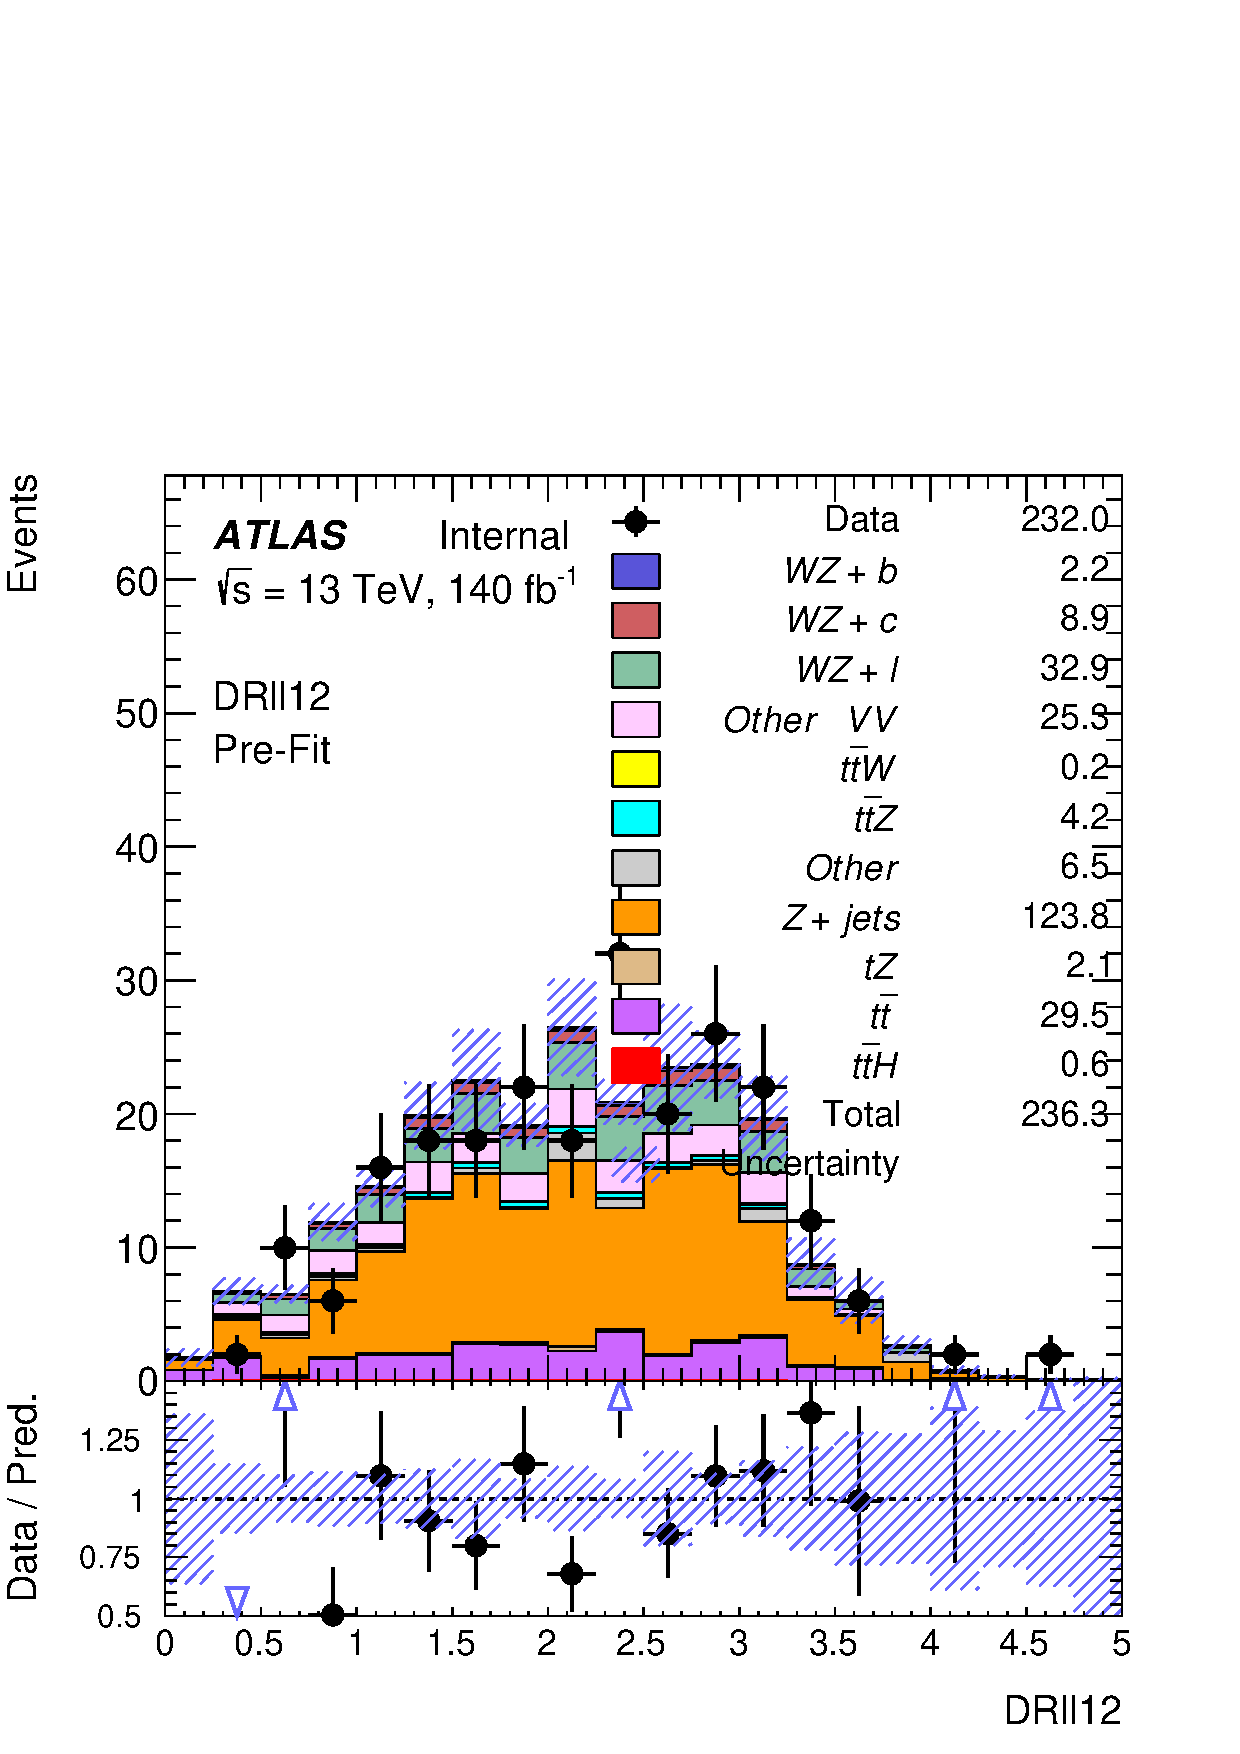
\includegraphics[width=.32\linewidth]{tZ_bdt_ab127/1j/ab127/DRll12.pdf}}\\
    
    \caption{Distribution of input features of the BDT for signal (WZ) and background (tZ). Both are scaled to an equal number of events. (a), (b) and (c) show the $p_T$ of lepton 0, lepton 1, and the jet, (d) show the reconstructed top mass, (e) and (f) show the invariant mass of leptons 0 and 1, leptons 0 and 2. (g) shows the $E_T^miss$ of each event. (h) and (i) show the $\Delta R$ between lepton 0 and lepton 1, and the jet.}
    \label{fig:tZ_kinematics}
\end{figure}

A sample of 20,000 background (tZ) and signal (WZ+b) Monte Carlo events are used to train the BDT. And additional 5,000 events are reserved for testing the model, in order to prevent over-fitting. A total of 750 decision trees with a maximum depth of 6 branches are used to build the model. These parameters are chosen empirically, by training several models with different parameters and selecting the one that gave the best separation for the test sample. 

The results of the BDT training are shown in figure \ref{fig:tZ_bdt}. The output scores for both signal and background events is shown on the left. The right shows the receiving operating characteristic (ROC) curve that results from the MVA. The ROC curve represents the background rejection as a function of signal efficiency, where each point on the curve represents a different response score. The ROC curve of the BDT is compared to the performance of using an optimal set of flat selections on the same set of input variables.

\begin{figure}[H]
\center
    \subfigure[]{\includegraphics[width=.45\linewidth]{tZ_bdt/xgb_score.png}}%
    \subfigure[]{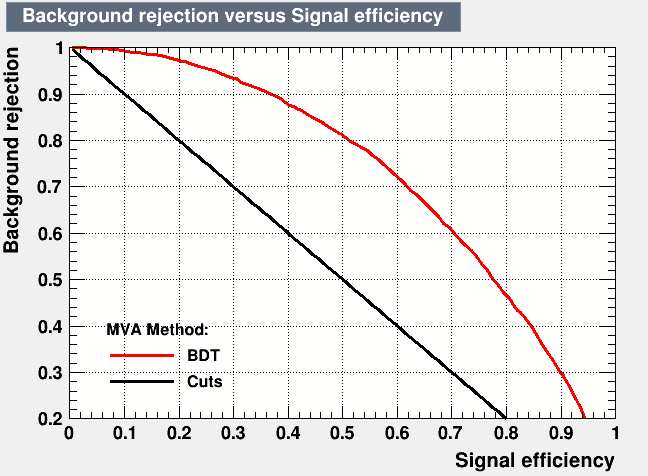
\includegraphics[width=.45\linewidth]{tZ_bdt/roc.png}}    
    \caption{Distribution of the BDT response for signal and background events on the left, the ROC curve for the BDT on the right.}
    \label{fig:tZ_bdt}
\end{figure}

The relative important of each input feature in the model, measured by how often they appeared in the decision trees, is shown in figure \ref{fig:tZ_fImp}.

\begin{figure}[H]
\center
        \includegraphics[width=0.9\linewidth]{tZ_bdt/feature_importance.png}
        \caption{Relative importance of each input feature in the model.}
        \label{fig:tZ_fImp}
\end{figure}

These results suggest that some amount of separation can be achieved between these two processes, with a high BDT score selecting a set of events that is pure in $WZ$ + b. 

